\documentclass[11pt, oneside]{article}   	% use "amsart" instead of "article" for AMSLaTeX format
\usepackage{tikz}
\usetikzlibrary{shapes,arrows}
\usepackage{geometry}                		% See geometry.pdf to learn the layout options. There are lots.
\usepackage{cancel}
\usepackage{marginnote}
\usepackage{mathtools}
\geometry{letterpaper}                   		% ... or a4paper or a5paper or ... 
\usepackage{graphicx}				% Use pdf, png, jpg, or eps� with pdflatex; use eps in DVI mode
								% TeX will automatically convert eps --> pdf in pdflatex		
\usepackage{amssymb}
\usepackage{bm}                                       % The 2 Following Liens Allows Matrix Notation
\newcommand{\matrva}[1]{\bm{#1}} 

\tikzstyle{block} = [draw, rectangle, 
    minimum height=3em, minimum width=4em]
\tikzstyle{sum} = [draw, circle, node distance=1cm]
\tikzstyle{input} = [coordinate]
\tikzstyle{output} = [coordinate]
\tikzstyle{pinstyle} = [pin edge={to-,thin,black}]

\title{\vspace{-3.5cm}Lab 4 - Simulink and Non-Linear Modeling}
\author{Derek Black}
\date{\vspace{-5ex}}

\begin{document}
\maketitle

%% Introduction Section %%
\section{Introduction}
\begin{itemize}
\item The Motorlab won't be used in today's lab. Instead we will be making a simulation of the hardware in Simulink and compare results found from the friction lab
\item Simulink is different because it allows us to do non-linear simulations. Example, students might have noticed gravity has never been included in dynamic equations, it is modeled as a disturbance. Gravity can be added in with Simulink.
\item The simulations are setup like those from a block diagram. It is possible to model a system as a block diagram and then simulate it with Simulink
\end{itemize}

\section{The Model}

\[\frac{\theta(s)}{\theta_c(s)} = \frac{K_p k_t k_{dr}}{Js^2 + bs + K_p k_t k_{dr}}        \]

\begin{figure}[!htb]
\begin{center}
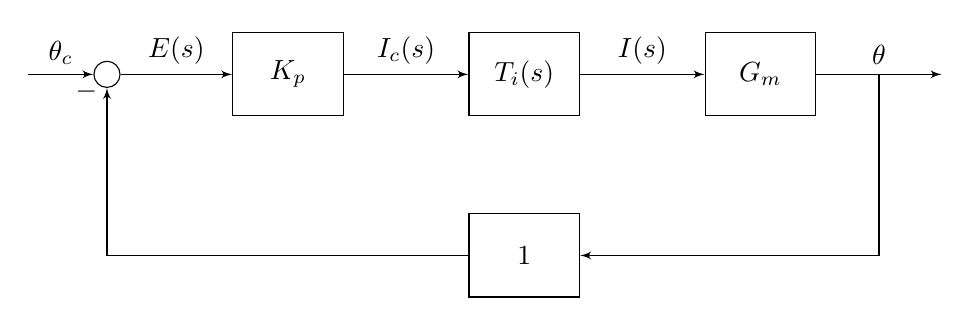
\begin{tikzpicture}[auto, node distance=2.3cm,>=latex']
    % We start by placing the blocks
    \node [input, name=input] {};
    \node [sum, right of=input] (sum) {};
    \node [block, right of=sum] (controller) {\(K_p\)};
    \node [block, right of=controller,
            node distance=3cm] (T) {\(T_i(s)\)};
     \node [block, right of=T,
            node distance=3cm] (system) {\(G_m \)};
    % We draw an edge between the controller and system block to 
    % calculate the coordinate u. We need it to place the measurement block. 
    \draw [->] (controller) -- node[name=u] {$I_c(s)$} (T);
    \draw [->] (T) -- node[name=u] {$I(s)$} (system);
    \node [output, right of=system] (output) {};
    \node [block, below of=T] (measurements) {1};

    % Once the nodes are placed, connecting them is easy. 
    \draw [draw,->] (input) -- node {$\theta_c$} (sum);
    \draw [->] (sum) -- node {$E(s)$} (controller);
    \draw [->] (system) -- node [name=y] {$\theta$}(output);
    \draw [->] (y) |- (measurements);
    \draw [->] (measurements) -| node[pos=0.99] {$-$} 
        node [near end] {} (sum);
\end{tikzpicture}
\end{center}
\end{figure}

\newpage
%% Second Section %%
\section{Introduction to Simulink}
\begin{itemize}
\item Simulink and MATLAB are dynamically linked together
\item This means Simulink can see changes to the workspace in MATLAB
\item This also means Simulink can output variables the MATLAB workspace that can be read
\end{itemize}


\subsection{Develop Simple Models in Simulink}
To illustrate how simulink works, demonstrate a few examples
\begin{enumerate}
\item Run setup.m file
\item To open simulink, type 'simulink' in the command window
\item Open the library browser. This is where all the different blocks are located
\item Continuous time blocks are were you can find things like the transfer function, etc.
\item Sinks are exactly what the name implies. Scopes, to workspace variables etc.
\item Sources are things like step inputs, sin waves etc.
\end{enumerate}
\subsubsection{Open Loop Model}

\begin{figure}[!htb]
\begin{center}
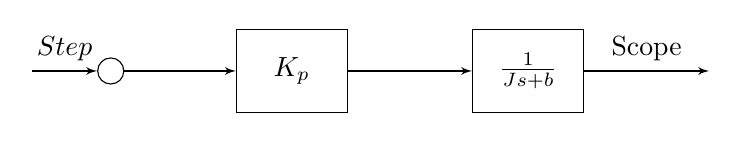
\begin{tikzpicture}[auto, node distance=2.3cm,>=latex']
    % We start by placing the blocks
    \node [input, name=input] {};
    \node [sum, right of=input] (sum) {};
    \node [block, right of=sum] (controller) {\(K_p\)};
    \node [block, right of=controller,
            node distance=3cm] (T) {\(\frac{1}{Js + b}\)};
    % We draw an edge between the controller and system block to 
    % calculate the coordinate u. We need it to place the measurement block. 
    \draw [->] (controller) -- node[name=u] {$$} (T);
   % \draw [->] (T) -- node[name=u] {$$} (output);
    \node [output, right of=T] (output) {};

    % Once the nodes are placed, connecting them is easy. 
    \draw [draw,->] (input) -- node {$Step$} (sum);
    \draw [->] (sum) -- node {$$} (controller);
    \draw [->] (T) -- node [name=y] {Scope}(output);
\end{tikzpicture}
\end{center}
\end{figure}

\subsubsection{Closed Loop Model}

\begin{figure}[!htb]
\begin{center}
\begin{tikzpicture}[auto, node distance=2.3cm,>=latex']
    % We start by placing the blocks
    \node [input, name=input] {};
    \node [sum, right of=input] (sum) {};
    \node [block, right of=sum] (controller) {\(K_p\)};
    \node [block, right of=controller,
            node distance=3cm] (T) {\(\frac{1}{J}\)};
     \node [block, right of=T,
            node distance=3cm] (system) {\(\frac{1}{s}\)};
    % We draw an edge between the controller and system block to 
    % calculate the coordinate u. We need it to place the measurement block. 
    \draw [->] (controller) -- node[name=u] {$$} (T);
    \draw [->] (T) -- node[name=u] {$$} (system);
    \node [output, right of=system] (output) {};
    \node [block, below of=T] (measurements) {b};

    % Once the nodes are placed, connecting them is easy. 
    \draw [draw,->] (input) -- node {$Step$} (sum);
    \draw [->] (sum) -- node {$$} (controller);
    \draw [->] (system) -- node [name=y] {$Scope$}(output);
    \draw [->] (y) |- (measurements);
    \draw [->] (measurements) -| node[pos=0.99] {$-$} 
        node [near end] {} (sum);
\end{tikzpicture}
\end{center}
\end{figure}

\section{Other useful information}

	\subsection{The First Simulation}
		\begin{itemize}
		\item The first simulation what you are doing is looking at the initial condition response that was done in the friction lab. However this time we are simulating the motorlab rather than actually running in on the hardware.
		\item Top block diagram is the actual motorlab simulation
		\item Bottom block diagram is the linear estimate for friction that we came up with
		\item There is an error somewhere in linear block diagram you have to find.
		\end{itemize}
		
	\subsection{The Second Simulation}
		\begin{itemize}
		\item The only two things that need to be done for the second simulation are: Putting in the transfer function block for the linear position control diagram.
		\item The second thing you are doing is putting the controller gains into the Nonlinear position control simulation
		\end{itemize}
		
	\subsection{Other things}
		\begin{itemize}
		\item Order of blocks matters. Remember different blocks emit different signals
		\item Ex. The controller block (i.e. Kp) emits a current.
		\item For the nonlinear position control simulation, notice we are asking you to saturate the current
		\item On the real motorlab system, the motor amplifier saturates the current at +- 3 amps. You need to incorporate that in your simulation using the saturation block.
		\item Explain why friction is a feeback term.
		\item Explain why there is a saturation block in the feedback
		\end{itemize}


\end{document}  